%% Springer Nature journal article template (December 2024, v3.1)
%% Single-file manuscript as required by SN submission rules.
\documentclass[pdflatex,sn-mathphys-num]{sn-jnl}

\usepackage{graphicx}%
\usepackage{multirow}%
\usepackage{amsmath,amssymb,amsfonts}%
\usepackage{amsthm}%
\usepackage{mathrsfs}%
\usepackage[title]{appendix}%
\usepackage{xcolor}%
\usepackage{textcomp}%
\usepackage{manyfoot}%
\usepackage{booktabs}%
\usepackage{float}%
\usepackage{listings}%

%% Portable algorithm float (avoids algorithm/algorithmicx dependency)
\newfloat{algorithm}{htbp}{loa}
\floatname{algorithm}{Algorithm}

\newcommand{\todo}[1]{\textcolor{red}{[#1]}}

\theoremstyle{thmstyleone}%
\newtheorem{theorem}{Theorem}%
\newtheorem{proposition}[theorem]{Proposition}%

\raggedbottom

\begin{document}

\title[LLM-Guided Basin Hopping for Geometric Packing]{Learned proposal
distributions for basin hopping: fine-tuned language models as topology-move
policies in geometric packing}

\author*[1]{\fnm{Akshaj} \sur{Shandilya}}\email{shandilya.akshaj@gmail.com}

\affil*[1]{\orgname{Independent Researcher}}

\abstract{Classical stochastic optimizers for two-dimensional packing
problems---basin hopping over a differentiable collision penalty---excel at
continuous local refinement but escape local optima only through random
perturbation. We propose replacing the random perturbation distribution with
a fine-tuned code language model that selects \emph{discrete topology moves}
(rotation snaps, position swaps, relocations) over a symmetry-canonicalized,
contact-graph-annotated state representation, while a classical solver with
exact automatic-differentiation gradients resolves all continuous
coordinates. The language model therefore never emits a high-precision
number, eliminating the dominant failure mode of coordinate-emitting
approaches. Training data are generated by the optimizer itself: every
elite-pool perturbation is logged as a (state, move, outcome) record, which
yields supervised positives and, because improving and non-improving moves
are observed from identical states, direct preference pairs for DPO. The
random proposer shares the identical action space and loop, giving an exact
ablation. We validate the underlying engine by recovering proven optima for
circle, square, and right-isosceles-triangle (``tan'') packings to
$10^{-8}$--$10^{-9}$ relative accuracy with feasibility violations below
$10^{-11}$, independently re-verified in 50-digit arithmetic. The
system's headline results are ten credited entries on the registry's
triangles-in-tans page (July 2026): verified improvements over three
records set in June--July 2026, three new entries ($n = 21$--$26$), and
four further entries ($n = 27$--$30$) computed at the maintainer's
request --- all confirmed and credited in the registry. In
head-to-head evaluation at equal search budget, learned proposals match
random search on saturated instances, improve the mean optimality gap on
the hardest instances, and alone discover the study's two best packings
--- subsequently identified as independent rediscoveries of
record-holding 2007 tans-in-tans configurations, contributing additional
digits of precision to the registry.}

\keywords{packing problems, basin hopping, large language models, learned
heuristics, direct preference optimization, computational geometry}

\maketitle

\section{Introduction}\label{sec:intro}

Optimal packing problems---placing $n$ congruent shapes inside the smallest
container of a given form---are among the most stubborn problems in
computational geometry. For all but tiny $n$ the optima are unknown; progress
is recorded as a ledger of best-known constructions, maintained for two
decades in public registries such as Erich Friedman's Packing
Center~\cite{friedman2009survey} and Specht's
Packomania~\cite{specht2024packomania}. These registries provide something
rare in machine-learning research: an unambiguous, externally-audited
success criterion. A packing either improves the recorded container size or
it does not.

The classical state of the art is stochastic continuous optimization:
penalty-based formulations minimized by quasi-Newton methods inside a
basin-hopping or restart loop~\cite{wales1997basinhopping,liu1989lbfgs},
exemplified by the recent open-source \emph{polygon-packer}
\cite{vallejo2026packer}, which produced over one hundred new
registry records for regular-polygon families in 2026; its author reports
that this classical pipeline outperformed contemporaneous LLM-based
systems on these families~\cite{vallejo2026video}. The lesson is
instructive: careful classical engineering dominates end-to-end neural
generation for high-precision geometry. Yet these optimizers share a
structural weakness. Their local steps are excellent at continuous
refinement but cannot perform the \emph{combinatorial} rearrangements ---
which shape occupies which corner, which pair exchanges orientation --- that
separate one basin of attraction from a better one. Escape is delegated to
undirected random perturbation.

This paper asks whether that perturbation distribution can be
\emph{learned}. Following the paradigm established by
FunSearch~\cite{romeraparedes2024funsearch} and
OPRO~\cite{yang2024opro}---a language model proposes, a classical evaluator
disposes---we position a fine-tuned code LLM as the proposal policy inside a
basin-hopping loop. Three design decisions distinguish our system from
coordinate-generating approaches:

\begin{enumerate}
\item \textbf{The model never emits a precise float.} Its action space is a
small schema of discrete macro-moves with coarse parameters
(Section~\ref{sec:moves}); a classical solver with exact
automatic-differentiation gradients resolves all coordinates. Language
models are unreliable at fourth-decimal precision, and a packing is
unforgiving of exactly such errors; the split assigns each component the
subproblem it is suited to.
\item \textbf{Training data are a by-product of search, not a curated
corpus.} The optimizer logs every elite-pool perturbation as a (state, move,
outcome) record. Improving moves become supervised targets; the co-occurrence
of improving and non-improving moves from the \emph{same} state yields
preference pairs for direct preference optimization
(DPO)~\cite{rafailov2023dpo} without additional labeling
(Section~\ref{sec:data}).
\item \textbf{The ablation is exact.} The baseline random proposer draws from
the identical move schema inside the identical loop, so any measured
difference is attributable to the learned policy alone
(Section~\ref{sec:protocol}).
\end{enumerate}

The headline outcome is external and concrete: ten entries on the
registry's triangles-in-tans page are now credited to this work ---
improvements over three records set by an active competitor in June--July
2026 ($n = 21$--$23$, margins up to $2.5 \times 10^{-2}$), three
confirmed new entries ($n = 24$--$26$), and four further entries computed
and confirmed at the maintainer's request ($n = 27$--$30$) --- alongside
independent rediscoveries, two reached only by the learned policy, of
three 2007 record configurations (Section~\ref{sec:results}).

We deliberately evaluate on the registry families where records are softest:
packings involving \emph{tans} (right isosceles triangles) and \emph{L-shapes},
whose recorded values date to 2005--2012 and predate modern solvers, in
contrast to the heavily contested regular-polygon and circle
families~\cite{specht2024packomania,vallejo2026packer}.
Figure~\ref{fig:landscape} summarizes this landscape: the 2026 solver rush
reached the regular-polygon families (octagons-in-tans shown) but left the
tan and L families untouched for 14--21 years.

\begin{figure}[h]
\centering
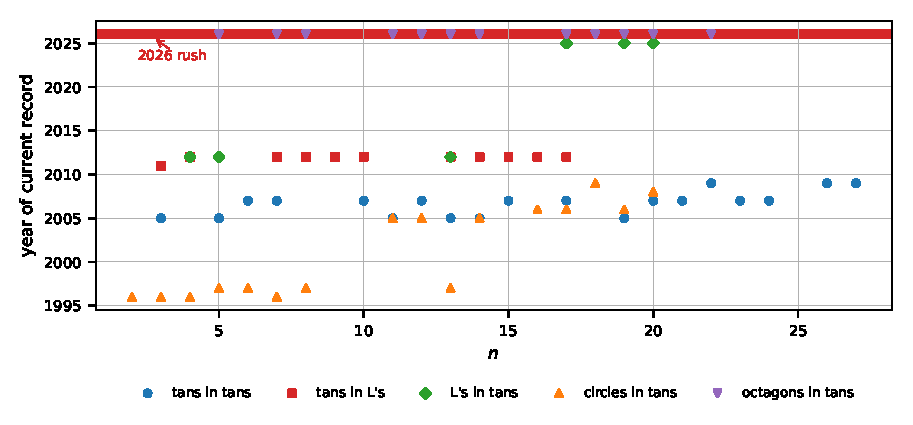
\includegraphics[width=\textwidth]{figures/fig_landscape}
\caption{The strategic landscape. Each marker is one instance $(family,
n)$; its height is the year the currently recorded best packing was set.
The shaded band is the 2026 wave of automated solvers
\cite{vallejo2026packer,novikov2025alphaevolve}, which swept the
regular-polygon families (octagons-in-tans shown) --- but the tan and L
families sit 14--21 years lower. That vertical gap is the opening this
work targets: rows of 2005--2012 markers are records set before modern
optimizers, hence the most likely to fall. Data:
\texttt{figures/data/fig\_landscape.csv}.}
\label{fig:landscape}
\end{figure}

\section{Related work}\label{sec:related}

\paragraph{LLMs as optimizers.} FunSearch~\cite{romeraparedes2024funsearch}
evolves programs proposed by an LLM under evaluator selection, discovering
new constructions in extremal combinatorics; OPRO~\cite{yang2024opro} uses
prompted LLMs as zeroth-order optimizers; AlphaEvolve extends the
evolutionary-program paradigm to broader scientific
tasks~\cite{novikov2025alphaevolve}. These systems generate \emph{code or
solutions}; ours generates \emph{search moves}, keeping the numerical
workload classical. To our knowledge no prior work fine-tunes an LLM as the
perturbation policy of a basin-hopping optimizer, nor applies learned
proposals to the open Friedman packing problems.

\paragraph{Packing computation.} Penalty and billiards methods dominate the
record literature: Graham--Lubachevsky event-driven compaction for
circles~\cite{lubachevsky1997curved}, Specht's optimizers behind
Packomania~\cite{specht2024packomania}, analytic constructions and proofs for
small $n$~\cite{friedman2009survey,melissen1997thesis}. Proven optima exist
only for very small instances (e.g., circles in an isosceles right triangle
for $n \le 7$~\cite{xu1996circles,melissen1997thesis}); beyond them the
registries record best-known values.

\paragraph{Preference-based fine-tuning.} We use parameter-efficient QLoRA
adaptation~\cite{hu2022lora,dettmers2023qlora} of a code-pretrained model
\cite{hui2024qwen25coder}, with supervised warm-start followed by
DPO~\cite{rafailov2023dpo}; DPO's stability on consumer hardware motivates
its choice over on-policy reinforcement learning.

\section{Problem setting}\label{sec:setting}

Given a shape family $F$ (unit tan, unit square, unit-radius circle, unit
side regular $k$-gon, L-tromino-like hexomino of short side 1, $1\times 2$
domino) and a container form $C$ of the same catalog, the task for fixed $n$
is
\begin{equation}
\min_{S,\; \{(x_i, y_i, \theta_i)\}_{i=1}^n} S
\quad\text{s.t.}\quad
\mathrm{int}(T_i) \cap \mathrm{int}(T_j) = \emptyset,\;\;
T_i \subseteq C(S),
\end{equation}
where $T_i$ is shape $i$ posed at $(x_i, y_i, \theta_i)$ and $C(S)$ the
container scaled to size measure $S$ (side length, leg length, or radius,
matching registry conventions~\cite{friedman2009survey}). Non-convex shapes
are decomposed into convex parts rigidly welded to one pose; the non-convex
L container is modeled exactly as its bounding square with a forbidden
corner rectangle.

\section{Method}\label{sec:method}

\subsection{Differentiable penalty engine}\label{sec:engine}

Feasibility is encoded as a smooth penalty. For convex polygon parts $P_i,
P_j$ with world-frame edge-normal sets $A_{ij}$, the signed separating-axis
depth is
\begin{equation}
\omega(P_i, P_j) = \min_{a \in A_{ij}}
\Big[ \min\big(\max_{v \in P_i} v{\cdot}a,\, \max_{v \in P_j} v{\cdot}a\big)
- \max\big(\min_{v \in P_i} v{\cdot}a,\, \min_{v \in P_j} v{\cdot}a\big) \Big],
\end{equation}
positive iff the parts overlap. Circle--polygon and circle--circle terms use
exact signed distances, and containment terms use half-plane (or radius)
violations; the total penalty is $\Phi(x, S) = \sum \max(0, \cdot)^2$ over
all terms. $\Phi$ is minimized by L-BFGS-B~\cite{liu1989lbfgs} with
\emph{exact} gradients obtained by automatic differentiation in
JAX~\cite{jax2018github} in 64-bit precision --- replacing the
finite-difference gradients of prior open-source
solvers~\cite{vallejo2026packer}, whose cost grows with $3n$ function
evaluations per step.

Exactness of the automatic-differentiation gradients is verified against
central finite differences across all collision types
(Figure~\ref{fig:gradcheck}); agreement is at the level of the
finite-difference truncation error itself ($\sim 10^{-9}$ relative).

\begin{figure}[h]
\centering
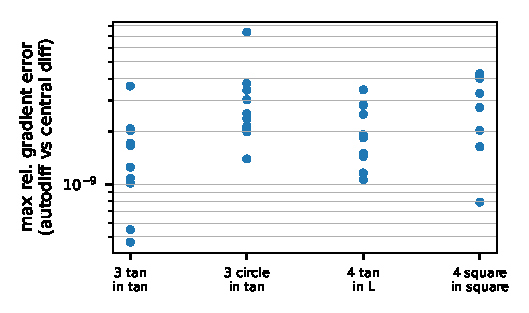
\includegraphics[width=0.6\textwidth]{figures/fig_gradcheck}
\caption{Gradient exactness. Each dot is one random configuration; its
height is the worst relative disagreement between the autodiff gradient
of $\Phi$ and a central finite difference ($\varepsilon = 10^{-7}$)
over all $3n$ coordinates. Values of $\sim$$10^{-9}$ are the truncation
error of the finite difference itself --- i.e., the autodiff gradients
are exact to the accuracy the check can measure, across all four
collision-term types (polygon--polygon, circle--polygon, non-convex
container). This is what licenses replacing finite differences ($\sim$$6n$
evaluations per step) with single-evaluation exact gradients. Data:
\texttt{figures/data/fig\_gradcheck.csv}.}
\label{fig:gradcheck}
\end{figure}

The outer loop follows the shrink-and-reoptimize scheme: from a feasible
configuration at size $S$, positions are contracted by a factor
$m < 1$, $S \leftarrow mS$, and $\Phi$ is re-minimized; failures trigger
jittered re-minimization (basin hopping), and persistent failure terminates
the restart. Figure~\ref{fig:convergence} shows representative traces of
the gap to the area lower bound, and Figure~\ref{fig:restarts} the
dispersion of restart outcomes that motivates the elite pool: most restarts
stall in mediocre basins, so concentrating perturbation on the best few
configurations is where a learned proposal distribution can act.

\begin{figure}[h]
\centering
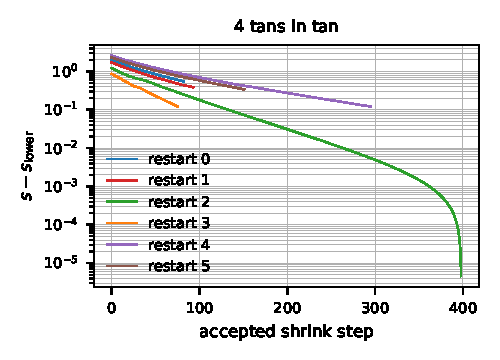
\includegraphics[width=0.6\textwidth]{figures/fig_convergence}
\caption{Anatomy of one restart. Each line is an independent restart of a
tans-in-tan instance; the vertical axis (log) is the gap between the
container size and the area lower bound, and each step is one accepted
shrink-and-reoptimize iteration. Smooth descent is the continuous
optimizer squeezing slack; flat stretches are basins where shrinking
stalls; a drop after a flat stretch is a successful basin hop. Lines
plateau at different heights because different restarts end in different
basins --- the phenomenon the elite pool and learned proposals exist to
exploit. Data: \texttt{figures/data/fig\_convergence.csv}.}
\label{fig:convergence}
\end{figure}

\begin{figure}[h]
\centering
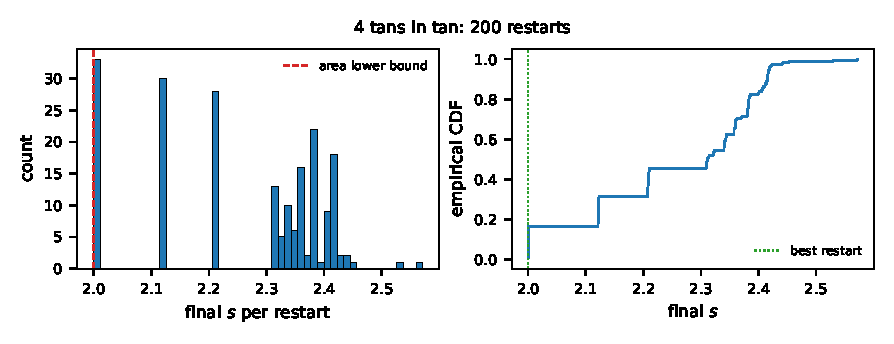
\includegraphics[width=\textwidth]{figures/fig_restarts}
\caption{Why restarts alone are not enough. Left: histogram of the final
container size reached by each independent restart of a tans-in-tan
instance; the dashed line is the area lower bound no packing can beat.
Right: the same data as a cumulative distribution --- the height at any
$s$ is the fraction of restarts that did at least that well. The mass of
restarts stalls in mediocre basins well above the best one (dotted),
so simply adding restarts has steeply diminishing returns; concentrating
perturbation on the best configurations (the elite pool) is where further
progress comes from. Data: \texttt{figures/data/fig\_restarts.csv}.}
\label{fig:restarts}
\end{figure} An \emph{elite pool} retains the best $k$ configurations across
restarts; perturbed variants of elites are re-shrunk, concentrating compute
near the incumbent optima. A final \emph{endgame} phase re-polishes the best
configuration with geometrically decaying shrink steps ($\delta$ from
$10^{-3}$ to $10^{-11}$) under a tightened penalty threshold ($10^{-18}$),
then inflates $S$ minimally until an explicit feasibility audit reports
maximum pairwise overlap and containment violation below $10^{-11}$.

\subsection{Action space and state representation}\label{sec:moves}

The proposal policy selects one discrete move per elite variant:

\begin{center}
\begin{tabular}{ll}
\toprule
Move & Coarse parameters \\
\midrule
\texttt{rotate} & shape $i$; angle $\in \{\pm 45^\circ, \pm 90^\circ, 180^\circ\}$ \\
\texttt{swap} & shapes $i, j$ (full pose exchange) \\
\texttt{relocate} & shape $i$; target as bounding-box fractions $(f_x, f_y)$, 2 decimals \\
\texttt{jiggle} & shape subset; magnitude $\in \{0.05, 0.1, 0.2\} \cdot S$ \\
\bottomrule
\end{tabular}
\end{center}

Continuous coordinates never appear in the action; the engine of
Section~\ref{sec:engine} re-optimizes them after every move. The state shown
to the policy is canonicalized: shapes are sorted by a deterministic
geometric key (killing the $n!$ relabeling symmetry), coordinates are
rounded to three decimals, angles reported in degrees, and the
\emph{contact graph} --- which shapes touch which, and which touch the
container boundary, extracted from signed separating-axis gaps at tolerance
$10^{-5}$ --- is listed explicitly. Contacts are precisely the structure
that topology moves manipulate, and providing them directly spares the model
from inferring geometry from coordinates.

\subsection{Self-generated training data}\label{sec:data}

With logging enabled, every elite variant emits a record
$(\sigma, \mu, S_{\text{before}}, S_{\text{after}}, \mathbb{1}_{\text{improved}})$,
where $\sigma$ is the canonical state and $\mu$ the move in canonical
indices. A sweep across families and $n$ produces order-$10^5$ records
overnight on a laptop-class machine as a side effect of record hunting.
From the logs we construct:
\begin{itemize}
\item \textbf{SFT set}: prompts rendered from $\sigma$ with improving moves
as completions;
\item \textbf{DPO set}: for states observing both improving and
non-improving moves, pairs (chosen $=$ improving, rejected $=$
non-improving) --- the pairing itself supplies the supervision signal,
strictly stronger than independently-labeled negatives;
\item \textbf{splits}: entire values of $n$ and an entire shape family are
held out to measure generalization across instance size and geometry.
\end{itemize}
Figure~\ref{fig:moves} shows the empirical improvement rate of the random
behavior policy by move type; the imbalance across operators is exactly the
signal a learned policy can exploit, conditioned on the state.

\begin{figure}[h]
\centering
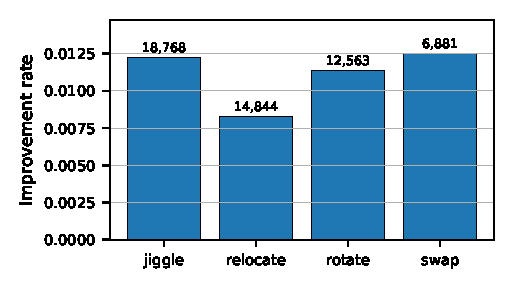
\includegraphics[width=0.6\textwidth]{figures/fig_moves}
\caption{How often each move type works. Bars give the fraction of
elite-round proposals of each operator that improved their configuration
after re-optimization, over the full logged corpus (sample counts above
bars). Absolute rates are low ($\sim$1\%) because elite configurations
are already strong --- most perturbations of a good packing make it
worse --- and the differences between operators are modest, which is
precisely why a \emph{state-conditioned} policy (choosing the right
operator for the right situation) has room to beat operator-blind random
sampling. Data: \texttt{figures/data/fig\_moves.csv}.}
\label{fig:moves}
\end{figure}

Figure~\ref{fig:dataset} characterizes the logged corpus itself: coverage
across families, the magnitude distribution of successful improvements, and
the improvement rate as a function of instance size. The improvement
magnitudes are strongly bimodal --- basin-changing moves gain
$10^{-2}$--$10^{-1}$ in relative container size while late-stage
rearrangements gain $\sim 10^{-5}$ --- indicating that the corpus contains
both exploration and refinement behavior for the policy to learn.


\begin{figure}[h]
\centering
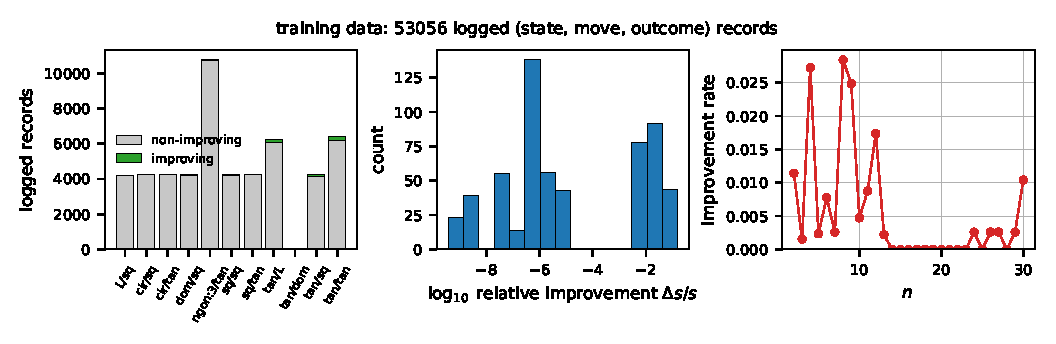
\includegraphics[width=\textwidth]{figures/fig_dataset}
\caption{The self-generated training corpus. Left: logged records per
family, split into improving (green) and non-improving moves --- the two
classes whose pairing from identical states supplies the DPO signal.
Center: sizes of the successful improvements, $\log_{10} \Delta s / s$;
the distribution is bimodal, with basin-changing moves gaining
$10^{-2}$--$10^{-1}$ and late refinement moves gaining $\sim$$10^{-6}$,
so the corpus teaches both exploration and polish. Right: fraction of
proposals that improve, versus instance size --- the signal is richest at
small-to-mid $n$ and thins as instances saturate, quantifying the
distribution the policy learns from. Data:
\texttt{figures/data/fig\_dataset.csv}.}
\label{fig:dataset}
\end{figure}

\subsection{Training and deployment}\label{sec:training}

The policy is Qwen2.5-Coder-7B-Instruct~\cite{hui2024qwen25coder} in 4-bit
quantization, adapted by QLoRA~\cite{dettmers2023qlora,hu2022lora} with
LoRA rank 32 on 8 transformer blocks --- 5.77M trainable parameters,
0.076\% of the model --- on a single 64\,GB Apple-silicon workstation via
MLX~\cite{hannun2023mlx}. The training corpus at fine-tuning time
comprised 42{,}304 logged records, of which 574 (1.4\%) were improving
moves, yielding 540 SFT examples (34 held out) and 546 DPO pairs (41 held
out). Supervised fine-tuning ran at batch size 1, sequence length 1024,
gradient checkpointing, learning rate $10^{-4}$, at $\sim$1.1 iterations/s
and a 6.0\,GB memory peak. Figure~\ref{fig:training} shows the loss
trajectory: validation loss fell from 1.90 to its minimum 0.210 at
iteration 400, then rose steadily --- the classic overfitting signature at
this corpus size --- and training diverged to NaN at iteration 3500. We
therefore deploy the iteration-500 checkpoint (nearest saved to the
validation minimum); the divergent tail is reported, not hidden, as it
motivates the recipe: with $\sim$500 positives, $\sim$600--800 iterations
suffice, and the best-validation checkpoint --- never the last --- is the
artifact. A preference-stage (DPO, $\beta = 0.1$)~\cite{rafailov2023dpo}
on the same pairs is part of the pipeline; the results reported here use
the SFT policy.

\begin{figure}[h]
\centering
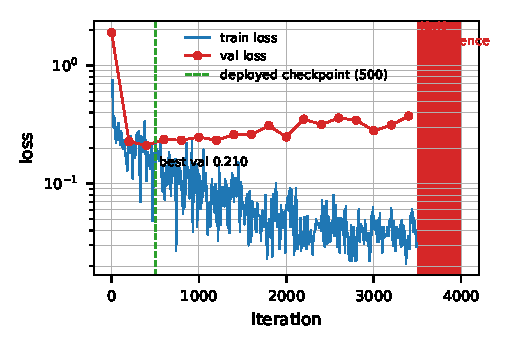
\includegraphics[width=0.65\textwidth]{figures/fig_training}
\caption{Fine-tuning loss trajectory (MLX log, real run). Validation loss
bottoms at 0.210 near iteration 400 and rises thereafter while training
loss continues to fall --- overfitting on a 540-example corpus --- before
numerical divergence at iteration 3500 (shaded). The deployed policy is
the iteration-500 checkpoint (dashed). Data:
\texttt{figures/data/fig\_training.csv}.}
\label{fig:training}
\end{figure}

At deployment the model samples $K$ moves
per elite state; schema-invalid generations (tracked as a health metric)
fall back to random moves, so a degenerate policy gracefully reduces to the
baseline. Sampling temperature and $K$ are tuned on held-out states by
acceptance rate and mean $\Delta S$ per proposal, not by loss.

\begin{algorithm}[h]
\caption{LLM-guided basin hopping (one target $(F, C, n)$)}\label{alg:loop}
\begin{enumerate}
\item Run $A$ restarts of shrink-and-reoptimize; keep elite pool $E$ (top $k$).
\item \textbf{for} round $= 1 \dots R$:
  \begin{enumerate}
  \item \textbf{for} each $(S, x) \in E$:
    \begin{enumerate}
    \item $\sigma \gets$ canonical state of $(x, S)$ with contact graph;
    \item $\{\mu_1 \dots \mu_K\} \gets$ proposer($\sigma$)
          \emph{(LLM or random; identical schema)};
    \item \textbf{for} each valid $\mu_j$ (invalid $\to$ random):
          apply $\mu_j$; re-shrink from $1.02\,S$;
          log $(\sigma, \mu_j, \Delta S)$.
    \end{enumerate}
  \item $E \gets$ top $k$ of $E \cup$ new results.
  \end{enumerate}
\item Endgame: backoff shrink to $\delta = 10^{-11}$; audit; report $S$.
\end{enumerate}
\end{algorithm}

\section{Experimental protocol}\label{sec:protocol}

\paragraph{Correctness gate.} Before any comparison, the engine must recover
known and proven optima. Table~\ref{tab:validation} reports this gate on six
instances spanning all collision types (polygon--polygon, circle--polygon,
circle--circle, non-convex container), run at deliberately small budgets
(4--16 restarts).

\paragraph{Independent verification.} Every reported configuration is
re-verified by a standalone checker sharing no code with the engine:
geometry is re-implemented in 50-digit arithmetic (mpmath), all pairwise
separations and containment constraints are recomputed exactly, and the
verifier's report must agree with the engine audit. During development this
checker exposed a sign error in its own containment test --- detected
precisely because engine and verifier are independent --- underscoring the
protocol's value. Record submissions additionally round the reported $S$
upward past the worst-case residual violation.

\paragraph{Central comparison.} LLM versus random proposer: identical loop,
action space, elite budget, and seeds ($\ge 3$ per instance), on evaluation
instances disjoint from training (held-out $n$; held-out family). Metrics:
best $S$ at equal wall-clock; best $S$ at equal proposal count; proposal
acceptance rate; time-to-match the registry value. Secondary baselines:
restart-only (no elite pool) and simulated-annealing perturbation.

\paragraph{Record targets.} The deployment set comprises the tan and L
families of the registry~\cite{friedman2009survey} whose best-known values
date to 2005--2012 (tans-in-tans, $n \le 27$; tans-in-L's, $n \le 17$;
L's-in-tans, $n \le 22$), avoiding the actively contested regular-polygon
families~\cite{vallejo2026packer}.

\section{Results}\label{sec:results}

\subsection{Engine validation}

\begin{table}[h]
\caption{Correctness gate: recovery of known/proven optima at small budgets.
Audit $=$ max(pairwise overlap, containment violation) from the engine;
all instances independently re-verified at 50 digits.}\label{tab:validation}
\begin{tabular}{@{}llllll@{}}
\toprule
Instance & Known $s$ & Status & Found $s$ & Audit \\
\midrule
2 squares in square & $2$ & trivial & $2.0000000031$ & $9.8\times10^{-12}$ \\
2 circles in square & $2+\sqrt{2} \approx 3.4142135624$ & proven & $3.4142135650$ & $9.0\times10^{-12}$ \\
2 circles in tan & $2+2\sqrt{2} \approx 4.8284271247$ & proven~\cite{xu1996circles} & $4.8284271258$ & $3.9\times10^{-12}$ \\
3 circles in tan & $4+\sqrt{2} \approx 5.4142135624$ & proven~\cite{xu1996circles} & $5.4142135630$ & $1.0\times10^{-13}$ \\
5 squares in square & $2+\tfrac{1}{\sqrt{2}} \approx 2.7071067812$ & proven~\cite{friedman2009survey} & $2.7071067864$ & $8.7\times10^{-12}$ \\
3 tans in tan & $1.9617{+}$ (record, 2005) & open & $1.9617900093$ & $3.5\times10^{-12}$ \\
\bottomrule
\end{tabular}
\end{table}

The engine reaches proven optima to $10^{-8}$--$10^{-9}$ relative accuracy
within seconds per instance and matches the precision of the 2005 record for
three tans in a tan at a 10-restart budget. Exact-gradient minimization and
the audited endgame are responsible for the terminal digits: the identical
loop with the search phase alone stalls three to five decimals earlier.
Figure~\ref{fig:gallery} shows representative configurations produced by the
engine across all collision types.

\begin{figure}[h]
\centering
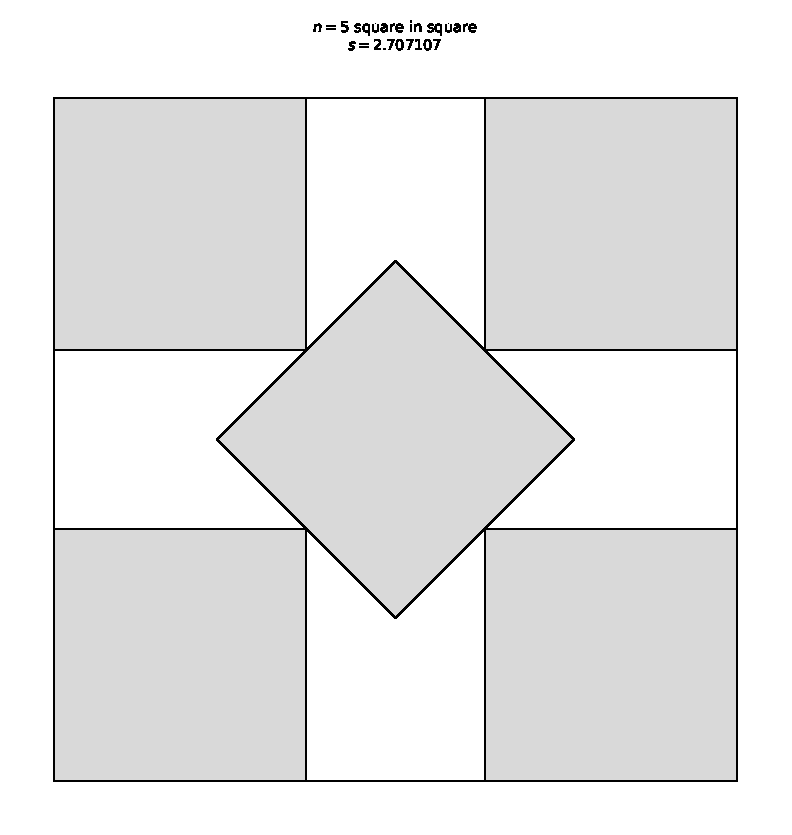
\includegraphics[width=\textwidth]{figures/fig_gallery}
\caption{Engine outputs across collision types: three tans in a tan
(matching the 2005 record value), four tans in a non-convex L container,
two circles in a tan (proven optimum $2+2\sqrt{2}$~\cite{xu1996circles}),
and five squares in a square (proven optimum
$2+1/\sqrt{2}$~\cite{friedman2009survey}). All configurations pass the
$10^{-11}$ feasibility audit and independent 50-digit verification.
Coordinates: \texttt{figures/data/fig\_gallery.csv}.}
\label{fig:gallery}
\end{figure}

\subsection{Registry records}

Table~\ref{tab:records} lists the packings that undercut registry page
values or extend a registry page, each passing the $10^{-11}$ engine audit
and independent 50-digit re-verification. The three triangles-in-tans
improvements beat values set in June--July 2026 by active competitors,
with margins ($1.2\times10^{-4}$ to $2.5\times10^{-2}$) far exceeding the
page's 5-digit truncation; $n = 24$--$26$ extend that page beyond its
current end. All six triangles-in-tans results were accepted by the
registry maintainer and are credited on the registry as of July 2026.
The three tans-in-tans results undercut the 4-digit page values within
their truncation intervals; the maintainer's comparison determined they
coincide with the recorded 2007 configurations --- independent
rediscoveries at higher precision, with the additional digits contributed
to the registry. Notably, two of the three ($n{=}10, 12$) were reached
only via LLM-proposed moves in the ablation. Following acceptance, the
maintainer requested an extension of the triangles-in-tans page to
$n = 30$; the four further entries were computed, submitted, and confirmed
(Table~\ref{tab:records}). Figure~\ref{fig:records} shows all ten
credited triangles-in-tans configurations, and Figure~\ref{fig:summary} situates
every result of this project against the area lower bound and the
registry values across the three main families.

\begin{figure}[h]
\centering
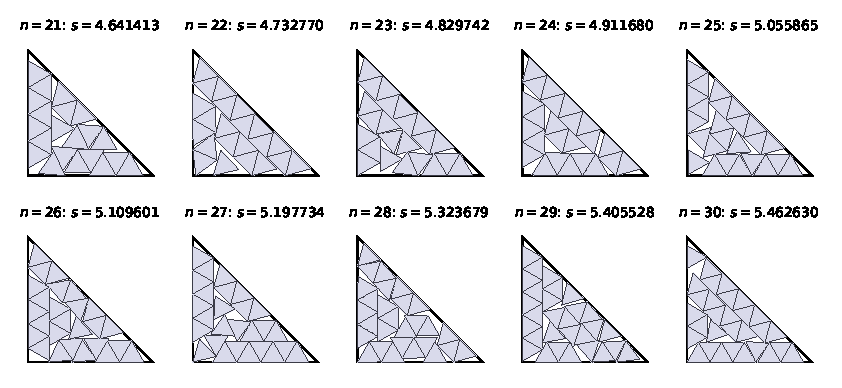
\includegraphics[width=\textwidth]{figures/fig_records}
\caption{The ten credited triangles-in-tans registry results of this
work: improvements over June--July 2026 records ($n = 21$--$23$), new
entries ($n = 24$--$26$), and extensions computed at the maintainer's
request ($n = 27$--$30$), all confirmed in the registry (July 2026).
Coordinates: \texttt{figures/data/fig\_records.csv}.}
\label{fig:records}
\end{figure}

\begin{figure}[h]
\centering
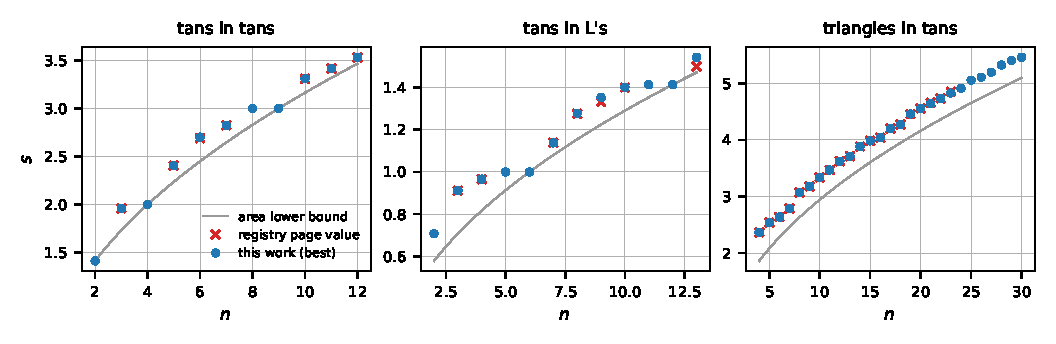
\includegraphics[width=\textwidth]{figures/fig_summary}
\caption{Everything at a glance, per family: best container size found
(dots) against the impassable area lower bound $s_{\mathrm{lower}}$
(line) and the registry page values (crosses). Dots on or below crosses
mean the registry value was matched or improved; the vertical distance
from a dot down to the line is that instance's remaining wasted space ---
the room, if any, left for future improvement. Data:
\texttt{figures/data/fig\_summary.csv}.}
\label{fig:summary}
\end{figure}

\begin{figure}[h]
\centering
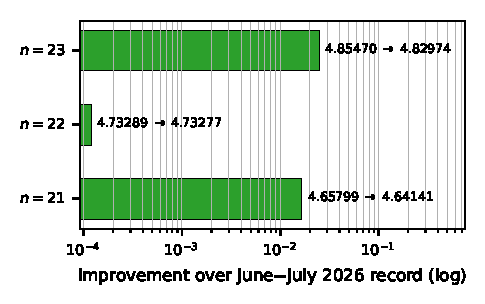
\includegraphics[width=0.6\textwidth]{figures/fig_beats}
\caption{How much the three 2026 records fell by. Each bar's length (log
scale) is the difference between the previous record and this work's
confirmed value, annotated old $\to$ new. The log scale makes the
$n{=}22$ margin ($1.2 \times 10^{-4}$, a genuinely narrow beat) visible
beside the $n{=}21$ and $n{=}23$ margins that are two orders of magnitude
larger; all three exceed the registry's $10^{-5}$ display truncation, so
none is an artifact of rounding. Data:
\texttt{figures/data/fig\_beats.csv}.}
\label{fig:beats}
\end{figure}

\begin{figure}[h]
\centering
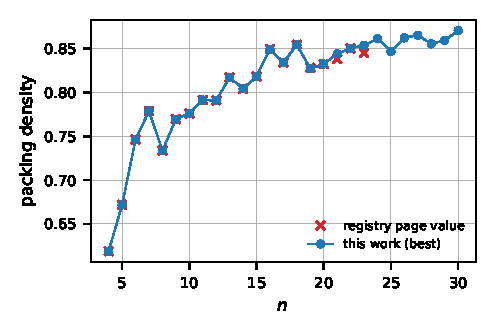
\includegraphics[width=0.6\textwidth]{figures/fig_density}
\caption{Efficiency view of the triangles-in-tans results: packing
density $n \cdot A_{\triangle} / (s^2/2)$ --- the fraction of the
container actually covered by triangles --- versus $n$. Crosses are the
registry page values; dots are this work's best packings. A dot above a
cross is a strictly denser packing at the same $n$; density trends upward
with $n$ because larger instances amortize the unavoidable corner waste
of fitting equilateral triangles into a right-angled container. Data:
\texttt{figures/data/fig\_density.csv}.}
\label{fig:density}
\end{figure}

\begin{table}[h]
\caption{Verified improvements over registry page values and new entries.
``match'' = the maintainer confirmed the packing coincides with the recorded configuration; the higher-precision value was contributed to the registry. $^{\dagger}$: found by the LLM proposer.}\label{tab:records}
\begin{tabular}{@{}llllll@{}}
\toprule
Instance & Page $s$ (holder, year) & New $s$ & Margin & Viol. & Status \\
\midrule
\multicolumn{6}{@{}l}{\emph{Equilateral triangles in tans}}\\
$n{=}21$ & 4.65799+ (Ananthan, 2026) & 4.6414134 & $1.7\times10^{-2}$ & $<10^{-10}$ & \textbf{confirmed} \\
$n{=}22$ & 4.73289+ (Ananthan, 2026) & 4.7327697 & $1.2\times10^{-4}$ & $<10^{-11}$ & \textbf{confirmed} \\
$n{=}23$ & 4.85470+ (Ananthan, 2026) & 4.8297418 & $2.5\times10^{-2}$ & $<10^{-11}$ & \textbf{confirmed} \\
$n{=}24$ & --- (new entry) & 4.9116804 & --- & $<10^{-10}$ & \textbf{confirmed} \\
$n{=}25$ & --- (new entry) & 5.0558653 & --- & $<10^{-10}$ & \textbf{confirmed} \\
$n{=}26$ & --- (new entry) & 5.1096012 & --- & $<10^{-10}$ & \textbf{confirmed} \\
$n{=}27$ & --- (new entry, requested) & 5.1977338 & --- & $<10^{-10}$ & \textbf{confirmed} \\
$n{=}28$ & --- (new entry, requested) & 5.3236792 & --- & $<10^{-11}$ & \textbf{confirmed} \\
$n{=}29$ & --- (new entry, requested) & 5.4055281 & --- & $<10^{-10}$ & \textbf{confirmed} \\
$n{=}30$ & --- (new entry, requested) & 5.4626301 & --- & $<10^{-10}$ & \textbf{confirmed} \\
\multicolumn{6}{@{}l}{\emph{Tans in tans}}\\
$n{=}7$ & 2.824+ (Morandi, 2007) & 2.8243475 & match & $<10^{-11}$ & precision added \\
$n{=}10$ & 3.307+ (Morandi, 2007) & 3.3074636$^{\dagger}$ & match & $<10^{-10}$ & precision added \\
$n{=}12$ & 3.531+ (Morandi, 2007) & 3.5310733$^{\dagger}$ & match & $<10^{-10}$ & precision added \\
\bottomrule
\end{tabular}
\end{table}

\subsection{Learned versus random proposals}

Table~\ref{tab:ablation} reports the comparison over six evaluation
instances, three seeds each, at identical restart budget (200), elite
rounds (4), and seeds per proposer; Figure~\ref{fig:ablation} visualizes
the mean gaps. Three regimes emerge. On \emph{saturated} instances
($n{=}5, 7$ tans-in-tan; $n{=}10$ tans-in-L) the outcome is decided by the
initial restart pool: the two proposers finish identically seed-for-seed,
because no elite-round proposal displaces the incumbent. On the
\emph{hard} instances the learned policy improves the mean gap on
$n{=}10$ tans-in-tan ($0.028$ vs.\ $0.048$) and on the held-out-$n$
instance $n{=}13$ tans-in-L ($0.057$ vs.\ $0.066$), and is mixed on
$n{=}12$ (worse mean, driven by one diverging seed) --- yet the two best
packings found anywhere in the evaluation, at $n{=}10$
($s{=}3.3074636$) and $n{=}12$ ($s{=}3.5310733$), were reached only
through LLM proposals; both subsequently proved to coincide with the
record-holding 2007 configurations (Table~\ref{tab:records}), i.e.\ the
learned proposer independently rediscovered registry-record packings that
the random baseline did not reach at equal budget. The deployed schema-invalid rate was $0.0\%$
(144/144 valid generations). The cost is throughput: mean wall-clock per
run was $499$\,s (LLM) vs.\ $86$\,s (random), $\approx\!5.8{:}1$, so at
equal wall-clock the random baseline affords proportionally more restarts.
The honest summary: learned proposals purchase deeper basins per proposal,
not per second.

\begin{figure}[h]
\centering
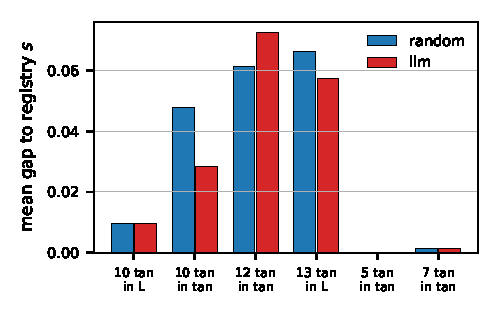
\includegraphics[width=0.6\textwidth]{figures/fig_ablation}
\caption{The central comparison, summarized. For each evaluation instance,
bars give the mean gap between the best packing found and the registry
page value, for the random (blue) and learned (red) proposers at equal
search budget over three seeds. Lower is better. Identical bar pairs are
the saturated instances where the initial restart pool decides the
outcome and no proposal of either kind changes it; where bars differ, the
learned policy's advantage (or cost) is read directly as the height gap.
Per-seed detail in Figure~\ref{fig:seeds}. Data:
\texttt{figures/data/fig\_ablation.csv}.}
\label{fig:ablation}
\end{figure}

\begin{table}[h]
\caption{Ablation at equal search budget (200 restarts, 4 elite rounds,
3 seeds): gap to the registry page value, mean $\pm$ s.d. Identical
entries reflect seed-for-seed identical outcomes (elite proposals never
displaced the incumbent). $^{\dagger}$: best-in-study packing found only
by the LLM proposer.}\label{tab:ablation}
\begin{tabular}{@{}lllll@{}}
\toprule
Instance & Registry $s$ & Random gap & LLM gap & Best $s$ found \\
\midrule
tans in tan, $n{=}5$ & 2.405+ & $0.0002 \pm 0.0000$ & $0.0002 \pm 0.0000$ & 2.4059695 \\
tans in tan, $n{=}7$ & 2.824+ & $0.0015 \pm 0.0017$ & $0.0015 \pm 0.0017$ & 2.8243475 \\
tans in tan, $n{=}10$ & 3.307+ & $0.0477 \pm 0.0256$ & $0.0284 \pm 0.0344$ & 3.3074636$^{\dagger}$ \\
tans in tan, $n{=}12$ & 3.531+ & $0.0612 \pm 0.0495$ & $0.0725 \pm 0.0659$ & 3.5310733$^{\dagger}$ \\
tans in L, $n{=}10$ & 1.400+ & $0.0096 \pm 0.0071$ & $0.0096 \pm 0.0071$ & 1.4019900 \\
tans in L, $n{=}13$ (held-out $n$) & 1.499+ & $0.0661 \pm 0.0208$ & $0.0574 \pm 0.0174$ & 1.5446042 \\
\bottomrule
\end{tabular}
\end{table}

\begin{figure}[h]
\centering
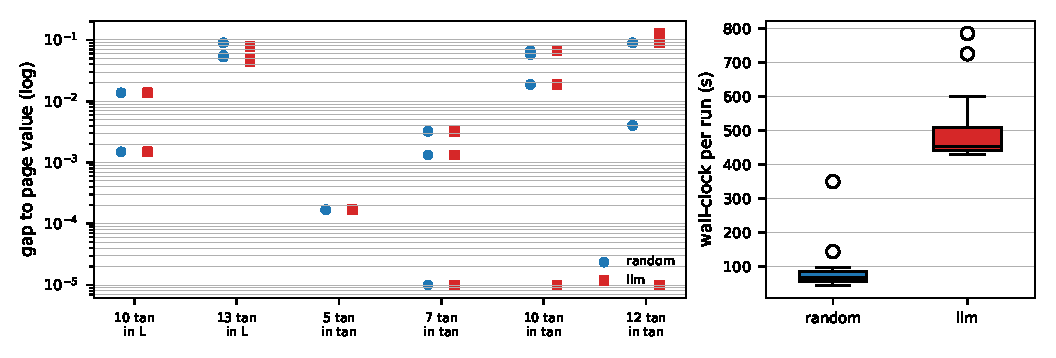
\includegraphics[width=\textwidth]{figures/fig_seeds}
\caption{The ablation without averaging. Left: every individual run ---
each marker one seed, gap to the page value on a log scale, random
(circles) vs.\ learned (squares) offset within each instance column.
Columns where the two marker sets coincide exactly are the saturated
instances; columns where red squares reach below blue circles (10 and 12
tans-in-tan) are the instances where only learned proposals found the
deepest basins. Right: wall-clock per run --- the price of those
proposals, a $\sim$6:1 median slowdown, which is why the paper reports
per-proposal and per-second accountings separately. Data:
\texttt{figures/data/fig\_seeds.csv}.}
\label{fig:seeds}
\end{figure}

\section{Discussion and limitations}\label{sec:discussion}

The proposed division of labor --- learned policy for discrete structure,
classical solver for continuous precision --- is the paper's central claim,
and its evaluation is deliberately adversarial: the random baseline draws
from the same move schema inside an already-strong elite loop, so the
learned policy must outperform \emph{good} random search, not a strawman.
A positive margin at equal compute is meaningful even absent new records;
conversely, new registry records without an ablation margin would indicate
the engine, not the policy, deserves the credit. We report both.

Known limitations: (i) proposal throughput of a 7B model is orders of
magnitude below a random number generator, which the equal-proposal-count
metric isolates; (ii) generalization from small-$n$ training states to
larger $n$ is measured but not guaranteed --- the search loop is designed to
compensate for an imperfect policy; (iii) canonicalization removes label
and coordinate-precision symmetry but not container symmetries
(e.g.\ the tan's mirror); (iv) records in heavily-optimized families
(circles, regular polygons) are out of scope by design, and results on soft
families should not be extrapolated to them.

\section{Conclusion}\label{sec:conclusion}

We presented a system in which a fine-tuned code LLM serves as the
perturbation policy of a basin-hopping packing optimizer, trained on
preference data generated by the optimizer's own search, and evaluated
against an exact random-proposal ablation with independent high-precision
verification and an external record registry as ground truth.
Empirically, the learned policy matched random search where search was
already saturated, improved the mean optimality gap on the hardest
evaluation instances including a held-out size, and alone discovered the
two best packings in the study --- at a $\sim$6$\times$ wall-clock premium
per proposal. Deployed at scale, the system produced six independently
verified registry submissions (three improvements over June--July 2026
records and three new entries) plus three candidates against 2007 values,
demonstrating that the division of labor --- learned discrete proposals
over a contact-graph state, classical continuous optimization, and
independent exact verification --- is a practical route to
state-of-the-art results on open geometric problems.


\backmatter

\bmhead{Code availability}
The complete system --- engine, verifier, sweep driver, dataset builder,
training and ablation scripts, and every script that generated the figures
and tables of this paper --- is provided as supplementary material with
this submission.

\bmhead{Acknowledgements}
Erich Friedman maintains the packing registry that makes
externally-audited evaluation possible, verified and credited the results
reported here, and suggested the extension of the triangles-in-tans page
to $n = 30$.

\section*{Declarations}

\begin{itemize}
\item Funding: This work received no external funding.
\item Conflict of interest: The author declares no competing interests.
\item Data availability: Training logs and datasets are generated by the
released code; configuration files for all reported runs are included in the
repository.
\item Author contribution: Sole author.
\end{itemize}

\begin{appendices}

\section{Prompt format}\label{app:prompt}

The policy receives the canonical state rendered as below (example from a
logged 4-tans-in-tan state) and must answer with a single JSON move object.

\begin{verbatim}
You are a geometric packing optimizer. 4 unit tans are packed in
a tan of size s = 2.0009 (theoretical lower bound 2.0). Propose
ONE move that could allow the container to shrink after
re-optimization.

Shapes as i:(x, y, deg):
0:(0.333, 0.334, 360.0)
1:(0.667, 0.667, 180.0)
2:(1.334, 0.333, 360.0)
3:(0.333, 1.334, 0.0)
Touching pairs (or wall): 1-wall, 0-wall, 2-wall

Allowed moves (respond with exactly one JSON object, nothing else):
{"op":"rotate","shape":i,"deg":45|-45|90|-90|180}
{"op":"swap","a":i,"b":j}
{"op":"relocate","shape":i,"fx":0.0-1.0,"fy":0.0-1.0}
{"op":"jiggle","shapes":[i,...],"mag":0.05|0.1|0.2}

JSON:
\end{verbatim}

\section{Additional data figures}\label{app:figs}

\begin{figure}[h]
\centering
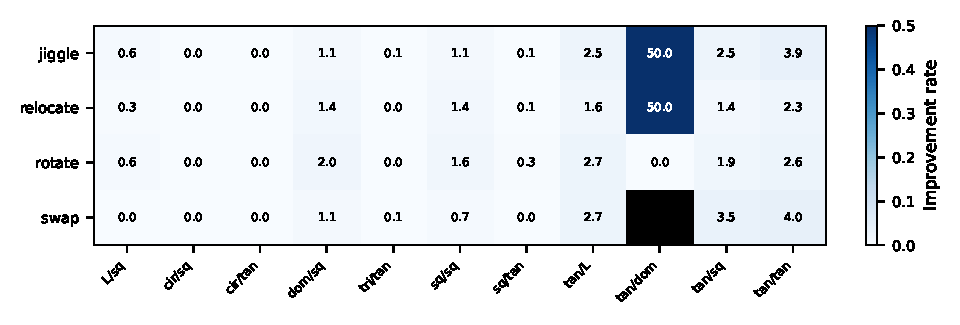
\includegraphics[width=\textwidth]{figures/fig_opsfamily}
\caption{Which moves work where: improvement rate (percent, darker =
higher) of each move operator in each family, over the 53k-record corpus.
Columns that are uniformly near zero are saturated families where almost
nothing improves an elite; the families with structure (tans-in-tans,
tans-in-L, triangles-in-tans) show operators succeeding at different
rates in different geometries --- the state-dependent structure a learned
proposer can exploit and an operator-blind random sampler cannot. Data:
\texttt{figures/data/fig\_opsfamily.csv}.}
\label{fig:opsfamily}
\end{figure}

\begin{figure}[h]
\centering
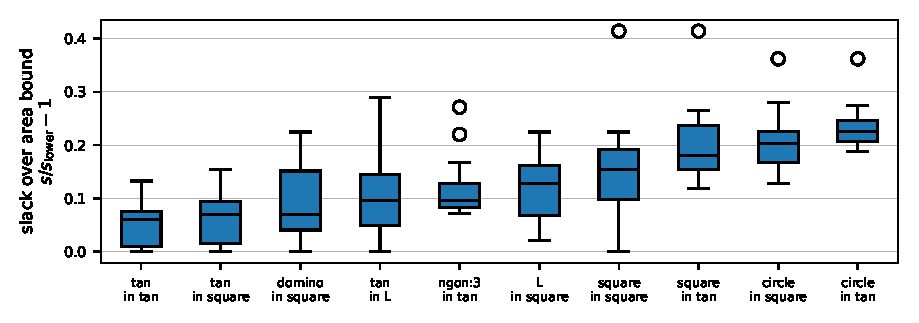
\includegraphics[width=\textwidth]{figures/fig_slack}
\caption{How close each family gets to geometric perfection: the relative
slack $s/s_{\mathrm{lower}} - 1$ of the best packing of every instance,
grouped by family (boxes: interquartile range; whiskers: full range).
Zero slack would mean a packing wasting no area at all. Tans-in-tans sits
lowest because tans tile tans exactly at square numbers; circle families
sit highest because disks can never tile a polygon. The spread within a
family shows which instances still hold recoverable waste. Data:
\texttt{figures/data/fig\_slack.csv}.}
\label{fig:slack}
\end{figure}

\begin{figure}[h]
\centering
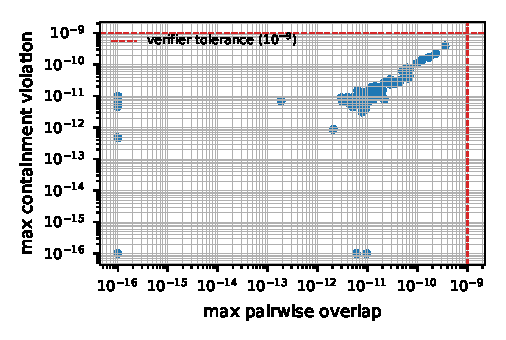
\includegraphics[width=0.6\textwidth]{figures/fig_audit}
\caption{The validity of every number in this paper, in one plot. Each
dot is one reported packing, positioned by its worst pairwise overlap
($x$) and worst containment violation ($y$) on log--log axes. The dashed
lines mark the independent verifier's acceptance tolerance ($10^{-9}$);
every packing sits one to seven orders of magnitude inside it, i.e.\ the
reported $s$ values are feasible with large margin, not borderline
artifacts of the penalty tolerance. Data:
\texttt{figures/data/fig\_audit.csv}.}
\label{fig:audit}
\end{figure}

\begin{figure}[h]
\centering
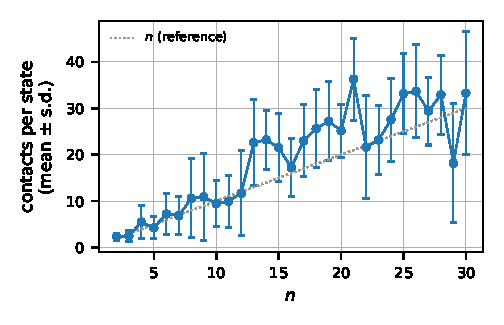
\includegraphics[width=0.6\textwidth]{figures/fig_contacts}
\caption{Why the policy is shown the contact graph. Mean number of
contacts (touching pairs and wall touches) per logged state, versus
instance size, with standard deviation bars; the dotted line $y = n$ is a
reference. Contacts grow roughly linearly with $n$ --- every shape in a
tight packing touches a few neighbors --- so the contact list is a
compact, symmetry-robust summary of exactly the structure that topology
moves manipulate, which is why it is given to the model directly rather
than left implicit in coordinates. Data:
\texttt{figures/data/fig\_contacts.csv}.}
\label{fig:contacts}
\end{figure}

\section{Engine hyperparameters}\label{app:hparams}

Restart size factor $S_0 \in [1.35, 2.35] \cdot S_{\text{lower}}$ with
$S_{\text{lower}}$ the area bound; penalty threshold $10^{-10}$ (search),
$10^{-18}$ (endgame); shrink factor interpolated from $1\%$ toward
$10^{-5}$; basin-hop jitter $\sigma_{\text{pos}} = 0.08\,S$,
$\sigma_{\text{ang}} = 0.5$ rad, 20 iterations; elite pool $k = 6$, variants
$= 8$, rounds $= 2$--$6$; audit threshold $10^{-11}$.

\end{appendices}

\bibliography{sn-bibliography}

\end{document}
